\section{Problem Formulation and Preliminaries}
\label{sec:mechanism}

\subsection{Posterior-Mean Representation}

Let \(n\) be a positive integer, \(X\) a uniform sign string in
\(\{-1,1\}^n\), and \(f\) a function from these strings to \(\{-1,1\}\).
Obtain \(Y\) by flipping
each bit with probability \((1-\rho)/2\). Correlation \(\rho=0\)
means complete noise; \(\rho=1\) means no noise. Define
\begin{align*}
 L&=\log2,\qquad h(r)=L-\phi(r),\\
 \phi(r)&=\frac{1+r}{2}\log(1+r)
          +\frac{1-r}{2}\log(1-r).
\end{align*}
Thus \(h(r)\) is the entropy of a sign-valued bit whose mean is \(r\).
In particular, \(h(0)=L\), \(h(\pm1)=0\), and
\(\phi'(r)=g(r):=\atanh r\).

For \(m=\E f\), write
\[
u(y)=T_\rho f(y)=\E[f(X)\mid Y=y].
\]
Constant rules retain no information, so only nonconstant \(f\) need
be studied. For these, \(-1<u(y)<1\) when \(0<\rho<1\), since
every input string has positive conditional probability.
The conditional probabilities of \(f(X)\) are \((1+u(y))/2\) and
\((1-u(y))/2\). The mutual information is therefore
\begin{equation}
 I_f(\rho)=h(m)-\E h(u)=\E\phi(u)-\phi(m).
 \label{eq:posterior-information}
\end{equation}
Every expectation without a subscript is uniform on the appropriate cube.
All logarithms are natural, so information is measured in nats.
This is the full-vector objective of Courtade and Kumar~\cite{CK}.
It differs from the two-Boolean-output objective settled in~\cite{PPM}
and the sum of coordinate informations bounded in~\cite{JW,Gemini}:
the conditional expectation above retains the entire observation \(Y\).

\begin{remark}[Dictator normalization]
If \(f(x)=x_1\), then \(m=0\), \(u(y)=\rho y_1\), and
\[
 I_f(\rho)=L-h(\rho)=\phi(\rho).
\]
The target is \(I_f(\rho)\le\phi(\rho)\). The parameter \(\rho\) is the
correlation, not the crossover probability.
\end{remark}

\begin{theorem}[Courtade--Kumar inequality]
\label{thm:CK}
For every positive integer \(n\), every Boolean function
\(f:\{-1,1\}^n\to\{-1,1\}\), and every \(0\leq\rho\leq1\),
\begin{equation}
 I(f(X);Y)\leq\phi(\rho).
 \label{eq:main-ck-sign}
\end{equation}
\end{theorem}

\subsection{Boolean Fourier Representation and Entropy Flow}

Write \([n]=\{1,\ldots,n\}\). For a subset \(S\subseteq[n]\), its
size is \(|S|\); the empty subset is \(\varnothing\).
Define \(\chi_S(x)=\prod_{i\in S}x_i\), with empty product one.
The Fourier coefficient of any cube function \(v\) is
\(\widehat v(S)=\E[v(X)\chi_S(X)]\).
The parity functions form an orthonormal
basis under the uniform measure. Thus
\[
 f=\sum_{S\subseteq[n]}\widehat f(S)\chi_S,\qquad
 \E f^2=\sum_S\widehat f(S)^2.
\]
A degree-\(|S|\) parity survives independent noise with factor
\(\rho^{|S|}\), so
\[
T_\rho f=\sum_S\rho^{|S|}\widehat f(S)\chi_S.
\]
This is the cube instance of the conditional-expectation spectral
viewpoint developed through principal inertia components in~\cite{PIC}.
Here we know each eigenvalue explicitly and keep its Fourier degree;
the standard Boolean Fourier facts used below are reviewed in~\cite{ODonnell}.
Define the cube Laplacian \(\Lapl \chi_S=|S|\chi_S\).
Write \(x^{\oplus i}\) for \(x\) with coordinate \(i\) flipped.
In physical coordinates,
\[
\Lapl v(x)=\frac12\sum_i\bigl(v(x)-v(x^{\oplus i})\bigr).
\]
Thus \(\Lapl \)
measures how a field differs from its neighbors, and also multiplies
each Fourier coefficient by its degree.
With \(y\) fixed, \(\partial_\rho u(y)\) denotes differentiating
the posterior \(u(y)=T_\rho f(y)\) with respect to \(\rho\).
This partial-derivative notation holds the other inputs fixed.
Differentiating the Fourier expansion shows that
\(\rho\,\partial_\rho u=\Lapl u\).
Likewise \(I_f'(\rho)=\frac{d}{d\rho}I_f(\rho)\) is the rate of change
of the scalar mutual information with \(f\) fixed.
Define the action, or rescaled information growth rate, by
\begin{equation}
 A(u):=\E[g(u)\Lapl u]=\rho I_f'(\rho).
 \label{eq:action}
\end{equation}
For a dictator, \(A=\rho g(\rho)\). The corresponding entropy-flow
identity is also central to Chen--Gohari--Nair~\cite[Lemma 1]{CGN};
we give the short derivation here to fix normalization.

The following monotone reduction removes changes of direction from the
subsequent edge analysis. It acts simultaneously at every noise level.

\begin{lemma}[Sorting preserves a possible advantage]\label{lem:sorting}
Every Boolean function can be replaced by a monotone Boolean function
in the same dimension, with the same mean and at least as much
information at every correlation.
\end{lemma}

\begin{proof}
Sort the function without decreasing its information. This reduction is due to
Courtade and Kumar~\cite{CK}; here is the argument in our notation.
In a chosen coordinate, the sections are the two functions
obtained by fixing that input bit to \(+1\) or \(-1\).
Let \(a\) be their average and \(b\) their half-difference, so
the sections are \(a+b,a-b\). Replace them by \(a+|b|,a-|b|\).
The mean is preserved. In this paragraph \(T\) denotes noise averaging
on the other coordinates at correlation \(\rho\).
After applying \(T\), the symmetric pair has half-separation
\(\rho Tb\), replaced by \(\rho T|b|\). Positivity gives
\(|Tb|\le T|b|\). For any convex function, its average at a symmetric
pair increases with the absolute separation. Thus sorting cannot
decrease \(I_f\), at any noise level. Min and max preserve previously
sorted coordinates, so sorting all coordinates leaves a monotone
function. Each sorting operation works simultaneously at all
correlations, so the same sorted function has the claimed advantage
throughout \([0,1]\).
\end{proof}

Here \emph{monotone} means that changing an input coordinate from \(-1\)
to \(1\) never decreases the output. The sorting step is what allows
Boolean structure to enter the next two lemmas.
Write \(\Delta_f(\rho)=I_f(\rho)-\phi(\rho)\) for the lead over
the dictator. It is continuous on \([0,1]\) and differentiable inside.
At the noiseless endpoint,
\[
 \Delta_f(1)=h(m)-\log2=-\phi(m)\le0.
\]
The proof will show that a positive lead must be increasing. Such a lead
cannot return to zero, contradicting this endpoint bound.
Unlike an optimizer analysis such as the clustering formulation
in~\cite{No}, this implication requires no stationarity of \(f\).
Unlike a proof confined to a high-noise neighborhood~\cite{Sam,YW},
its conclusion is used along a whole interval ending at the noiseless
endpoint. The inequalities below must supply that finite-range control.

Use one common boundary for the two arguments:
\[
                         \rho_*:=\tanh(31/20).
\]
For \(0\le\rho\le\rho_*\), Appendix~\ref{app:low} proves the
information bound at every bias, using the elementary Fourier estimate
in Section~\ref{app:fourier-cap-proof}. The growth argument below starts
at exactly the same boundary. Thus a positive lead must occur above
\(\rho_*\); no overlap between separately chosen ranges is needed.

\begin{figure}[ht]
\centering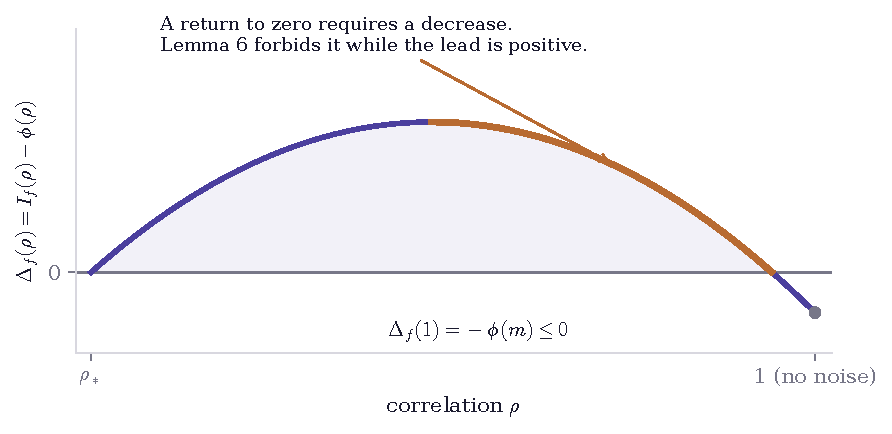
\includegraphics[width=.94\linewidth]{maximum.pdf}
\caption{Schematic of the growth contradiction. A positive lead would
have to decrease before reaching its nonpositive value at \(\rho=1\),
whereas Lemma~\ref{lem:coverage} shows that it is strictly increasing
whenever it is positive.}
\label{fig:growth-contradiction}
\end{figure}

For a putative violation, the information premise is exactly
\begin{equation}
 \E h(T_\rho f)<h(\rho)-\phi(m).                         \label{eq:premises}
\end{equation}
It supplies a positive credit in the spectral baseline. Our target is
\(A(u)>\rho\logodds\), with \(\logodds=\atanh\rho\):
by \eqref{eq:action}, this says that the lead is increasing.

\section{Edge Geometry and the Pivotal Decomposition}
\label{sec:edges}

For a coordinate index \(i\), let \(f_{i,+}\) and \(f_{i,-}\) be the
sections obtained by fixing that input to \(+1\) and \(-1\), respectively.
For a monotone Boolean function, the derivative in coordinate \(i\),
viewed on the other \(n-1\) coordinates, is
\[
 q_i^f=\frac{f_{i,+}-f_{i,-}}2\in\{0,1\}.
\]
It indicates a pivotal edge: one on which the output changes.
The influence \(\Inf_i(f)\) is the probability of such an edge.
Its mean
\[
 a_i=\E q_i^f=\widehat f(\{i\})=\Inf_i(f)
\]
is both the singleton Fourier coefficient and the influence.
This identity is special to monotone Boolean functions. After noise,
\(\E(u_{i,+}-u_{i,-})/2=\rho a_i\).
For a dictator, \(f_{1,+}=1\) and \(f_{1,-}=-1\), so
\(q_1^f=1\) everywhere; every other \(q_i^f\) is zero.
Retaining the indicator \(q_i^f\), rather than just its mean, will be
essential. Moment relaxations of the posterior can admit objects that
are not Boolean noise images, a distinction also examined
in~\cite[Section 8.1.2]{Gemini}. Our logarithmic Sobolev step acts on
the actual pivotal indicator and its positive smoothings.

For an edge with endpoint values \(p,q\), the action and angle energy
contributions are
\begin{align*}
 a(p,q)&=\frac{(p-q)(g(p)-g(q))}{4},\\
 j(p,q)&=\frac{(\arcsin p-\arcsin q)^2}{4}.
\end{align*}
Average over the edges in each coordinate direction, then sum over
directions. The results are \(A(u)\) and
\(\E[\Theta \Lapl \Theta]\), with \(\Theta=\arcsin u\).
Cauchy--Schwarz gives \(a\ge j\). We need a stronger statement which
keeps track of the difference.

\begin{remark}[Angular parametrization]
The derivative of \(g\) is \(g'(r)=1/(1-r^2)\).
Its square root is the derivative of \(\arcsin r\). For \(p\ge q\),
\[
 \left(\int_q^p\frac{\diff r}{\sqrt{1-r^2}}\right)^2
 \le (p-q)\int_q^p\frac{\diff r}{1-r^2}.
\]
This is exactly \(j(p,q)\le a(p,q)\). The angle turns an edge's
information cost into a squared difference, which Fourier analysis can
handle. The lemma retains the cost left over in this conversion.
\end{remark}

Define
\[
 F(v)=\frac{h(\tanh v)}{\tanh v},\qquad
 c(v)=\frac{\arcsin(\tanh v)^2}{\tanh v}.
\]
The function \(F\) decreases from infinity to zero. An entropy budget
\(H_{\rm budget}>0\) sets the centered comparison pair for each active
coordinate: its values are \(\pm\tanh v_i\), where
\[
                    F(v_i)=\frac{H_{\rm budget}}{\rho a_i}.
\]
This matches entropy per unit width. The comparison height \(v_i\)
is not a posterior observed on an individual edge. A smaller entropy
budget gives a larger height and a stronger growth bound.

The first bound below is the entropy-constrained edge envelope of
Chen--Gohari--Nair~\cite[Theorem 4 and Appendix C]{CGN}, written for
signs and natural logarithms. We also need the angle correction,
whose derivation is supplied in Appendix~\ref{app:scalar}.
No conjectured inequality from that paper is assumed.
The difference from its potential-induction program is where the
remaining cost is paid: here the edge correction is combined with
Fourier information from the same Boolean rule.

The same centered comparison pair will control both the total growth and
the residual growth after subtracting the angle energy. Using a common
entropy budget in the two bounds is essential for combining them later.

\begin{lemma}[The edge budget]\label{lem:edges}
Let \(f\) be nonconstant and monotone, \(0<\rho<1\), and
\(u=T_\rho f\). Choose any entropy budget
\(H_{\rm budget}\ge\E h(u)>0\). For every coordinate with
\(a_i>0\), define \(v_i\) by
\(F(v_i)=H_{\rm budget}/(\rho a_i)\). Then
\begin{align}
 A(u)&\ge\rho\sum_i a_i v_i,                         \label{eq:edge-budget}\\
 A(u)&\ge\E[\Theta\Lapl\Theta]
           +\rho\sum_i a_i\bigl(v_i-c(v_i)\bigr).   \label{eq:correction}
\end{align}
Coordinates with \(a_i=0\) contribute zero and are omitted.
\end{lemma}

\begin{proof}
For one edge put \(\edgewidth=|p-q|/2\) and
\(H_e=[h(p)+h(q)]/2\). The notation \(F^{-1}\) means the inverse
of the decreasing profile \(F\), not its reciprocal. Define the
correction function \(\corr\) by \(\corr(F(v))=v-c(v)\).
The scalar calculation in Appendix~\ref{app:scalar} proves
\begin{align*}
 a(p,q)&\ge\edgewidth F^{-1}(H_e/\edgewidth),\\
 a(p,q)-j(p,q)&\ge\edgewidth\corr(H_e/\edgewidth).
\end{align*}
Both right sides are convex in \((\edgewidth,H_e)\) and decrease
with \(H_e\). For coordinate \(i\),
\(\E\edgewidth=\rho a_i\) and
\(\E H_e=\E h(u)\le H_{\rm budget}\).
Jensen therefore bounds the two averaged edge costs below by their
values at \((\rho a_i,H_{\rm budget})\). Their inverse parameter
is exactly \(v_i\). Summing over coordinates proves both claims.
\end{proof}

For a dictator, choose its actual entropy \(H_{\rm budget}=h(\rho)\).
Put \(\theta=\arcsin\rho\). The sole height is
\(v_1=\atanh\rho\), and the two conclusions become
\(A=\rho\atanh\rho\) and
\(A=\theta^2+(\rho\atanh\rho-\theta^2)\). Thus the lemma preserves the
complete edge account, including the positive correction.

We use this lemma with two budgets. Whenever \(\E h(u)\le h(\rho)\),
the choice \(H_{\rm budget}=h(\rho)\) defines heights \(\ell_i\) by
\begin{equation}
                    F(\ell_i)=F(\logodds)/a_i.       \label{eq:heights}
\end{equation}
Since \(a_i\le1\), these satisfy \(0<\ell_i\le\logodds\).
The middle argument will use a smaller budget that also retains the
output mean; the lemma applies without changing its proof.

For the following illustration only, \(v\) is an edge-center parameter
and \(k>0\) its half-width in inverse-hyperbolic-tangent coordinates:
\(p=\tanh(v+k)\), \(q=\tanh(v-k)\).
These are local plot parameters. The plotted \(\edgewidth ,H_e,j\) are the
edge half-separation, average entropy, and angle cost defined above.

\begin{figure*}[t]
\centering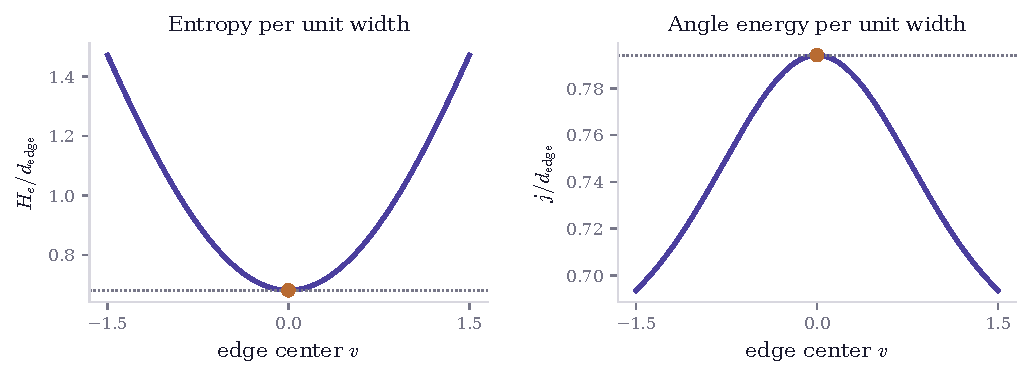
\includegraphics[width=.76\textwidth]{centered-edge.pdf}
\caption{The geometry behind the edge lemma. Write the endpoints as
\(p=\tanh(v+k)\), \(q=\tanh(v-k)\), with \(k=0.8\) in this illustration.
Centering at \(v=0\) minimizes entropy per unit width and maximizes
angle energy per unit width. These two extremal facts give a convex
lower bound on the action left after angle energy is removed.}
\label{fig:centered-edge}
\end{figure*}

With this budget, the first inequality bounds the total comparison weight:
\begin{equation}
                     W:=\sum_i a_i \ell_i\le A(u)/\rho.           \label{eq:W}
\end{equation}
For a dictator there is one active coordinate, \(a_1=1\), \(\ell_1=\logodds \),
and equality holds. The second inequality will be combined with a
spectral lower bound. Keeping its correction is essential.

\section{Information Growth Across Channel Regimes}
\label{sec:pivotal-middle}

\subsection{Intermediate-Correlation Growth}

We first prove the required growth inequality on the intermediate range
\(31/20\le\ell=\atanh\rho\le7/2\). In this section write \(r=\rho\).
The idea is to keep the coordinates together. Logarithmic Sobolev gives
an entropy cost for their pivotal probabilities; the log-sum inequality
then combines that cost with the edge budget. We will not choose a
comparison Fourier degree or divide coordinates by influence.
The underlying entropy tool is Gross's cube logarithmic Sobolev
inequality~\cite{Gross,ODonnell}. Its use here is specific: the positive
kernel in the next calculation converts pivotal-set entropy into the
same spectral expression produced by the centered angle comparison.
This supplies the correction left after the entropy-flow edge
bound~\cite{CGN}, without a conjectured coupling potential.


\begin{proposition}[Pivotal entropy forces faster growth]
\label{prop:middle-growth}
Let \(f\) be monotone Boolean and
\(31/20\le\atanh\rho\le7/2\). Then
\[
 I_f(\rho)>\phi(\rho)\quad\Longrightarrow\quad
 I_f'(\rho)>\phi'(\rho).
\]
The mean of \(f\) is unrestricted.
\end{proposition}

The proof compares the energy demanded by the information premise with
the growth available along the cube edges. It first obtains an
angle-energy requirement, expresses part of that requirement as pivotal
entropy, and then combines the entropy with the edge correction through
the log-sum inequality.

Put \(\Theta=\arcsin u\) and \(J_{\rm ang}=\E[\Theta\Lapl\Theta]\).
The dictator has posterior values \(\pm r\). Define its angle and the
slope of the line through those two angle values by
\[
 \theta=\arcsin r,\qquad \lambda=\theta/r.
\]
Two further coefficients come from the tangent inequality below:
\[
 \alpha=\frac{\theta+\sinh\ell}{\ell},\qquad
 \gamma=\lambda\alpha,\qquad
 \eta=\frac{\theta^2\gamma}{\gamma+1}.
\]
These are channel functions, not parameters to optimize.
The same \(\gamma\) will serve throughout the growth proof, including
the high-correlation extension. Only the way we estimate the pivotal
cost changes with the channel.

\subsubsection{Angle energy required by an information lead}

The following scalar inequality is proved in
Appendix~\ref{app:centered-support}:
\begin{equation}
 \begin{split}
 \frac{\alpha}{2}(\arcsin x-\lambda x)^2
 &\le x\arcsin x-r\theta\\
 &\quad-\alpha[\phi(x)-\phi(r)],qquad -1\le x\le1.
 \end{split}
 \label{eq:centered-support}
\end{equation}
Both sides vanish at \(x=\pm r\). It bounds the error of the
dictator's angle line by an entropy difference, without losing
equality at the reference posterior.
The comparison stays within Shannon entropy. Although the angle and
the Hellinger program~\cite{Hellinger,CN} both involve the geometry of
binary probabilities, we do not infer this inequality from a
Hellinger-optimality conjecture; its scalar proof is given in full.

Average \eqref{eq:centered-support} with \(x=u\), multiply by
\(2\lambda\), and complete the square in the positive operator
\(\Lapl+\gamma\). This gives
\begin{equation}
 \begin{split}
 J_{\rm ang}\ge{}&2\theta^2+2\gamma[\phi(m)+\Delta_f(r)]\\
 &+\lambda^2\E\left[u\left\{\gamma-
       \frac{(\gamma+1)^2}{\Lapl+\gamma}\right\}u\right].
 \end{split}
 \label{eq:centered-resolvent}
\end{equation}
Here division by \(\Lapl+\gamma\) means multiplication of each
degree-\(k\) Fourier coefficient by \(1/(k+\gamma)\).
For completeness, the discarded nonnegative square is
\begin{multline*}
 \E\bigl[
 \bigl(\Theta-\lambda(\gamma+1)(\Lapl+\gamma)^{-1}u\bigr)
 (\Lapl+\gamma)\\
 {}cdot\bigl(\Theta-\lambda(\gamma+1)
 (\Lapl+\gamma)^{-1}u\bigr)\bigr].
\end{multline*}
The constant Fourier mode is included; this matters when \(m\ne0\).
For the dictator, \(u=ry_1\) and \(\Theta=\lambda u\) are both
degree one. The operator \((\gamma+1)(\Lapl+\gamma)^{-1}\)
therefore fixes \(u\), so the discarded square is zero. In
\eqref{eq:centered-resolvent} the spectral term is \(-\theta^2\);
the result is exactly \(J_{\rm ang}=\theta^2\).

\subsubsection{Contribution of noisy pivotal sets}

Recall the pivotal indicator \(q_i^f\), with mean \(a_i\).
Omit coordinates with \(a_i=0\); every logarithm below then has a
positive argument.
Let \(t\in[0,r^2]\) denote a squared noise correlation and put
\[
 w_i(t)=T_{\sqrt t}q_i^f,\qquad s_i(t)=\E w_i(t)^2.
\]
Noise here acts on the other \(n-1\) coordinates.
The value \(w_i(t)\) is the conditional probability that coordinate
\(i\) is pivotal. Its mean remains \(a_i\); its second moment
\(s_i(t)\) records how unevenly that probability is distributed.
Complete averaging gives \(s_i(0)=a_i^2\), whereas the unsmoothed
indicator has second moment \(a_i\).
Define an average of these second moments:
\[
 z_i=\frac{\gamma+1}{\gamma r^2}
       \int_0^{r^2}[1-(t/r^2)^\gamma]s_i(t)\,dt,
 \qquad Z=\sum_i z_i.
\]
The weight in this integral is nonnegative and has total mass one.
Thus \(a_i^2\le z_i\le a_i\): noise preserves the mean and cannot
increase the second moment of an indicator.

Write \(V_0=1-m^2\) for the Boolean variance and
\(U=\operatorname{Var}(u)/r^2\) for the normalized noisy variance.
Fourier expansion of the integral gives
\[
 Z=(\gamma+1)\sum_{k\ge1}
       \frac{r^{2(k-1)}}{\gamma+k}
       \sum_{|S|=k}\widehat f(S)^2,
 \qquad 0<Z\le U\le V_0.
\]
The last inequality is Boolean Parseval followed by noise contraction.
For a dictator, \(w_1(t)=s_1(t)=z_1=1\), all other
coordinate terms vanish, and \(Z=U=V_0=1\). Thus \(V_0-Z\)
measures a variance reserve that is absent in the equality example.
The exact integral identity
\begin{align*}
 &\frac{\gamma+1}{\gamma}
 \int_0^{r^2}[1-(t/r^2)^\gamma]
       \sum_i\E[w_i(t)\Lapl w_i(t)]\,dt\\
 &\hspace{7em}=(\gamma+1)r^2(U-Z)
\end{align*}
is checked one Fourier degree at a time: a degree-\(k\) coefficient
appears in \(k\) pivotal derivatives, each of degree \(k-1\).

Cube logarithmic Sobolev, proved in Appendix~\ref{app:scalar}, gives
\[
 \E[w_i\Lapl w_i]\ge
       \frac12 s_i\log\frac{s_i}{a_i^2}.
\]
For the auxiliary entropy bound, average under the probability
density \(w_i^2/s_i\). Jensen applied to \(\log(1/w_i)\) gives
\(\E_*\log w_i\ge\log(s_i/a_i)\), hence
\(\operatorname{Ent}(w_i^2)\ge s_i\log(s_i/a_i^2)\).
Here \(\operatorname{Ent}(v)=\E(v\log v)-(\E v)\log(\E v)\);
zero-weight points are omitted. Convexity of \(s\log(s/a_i^2)\)
and the averaging integral therefore give a bound on the
\emph{pivotal entropy cost}, defined by
\[
 E_{\rm piv}:=\sum_i z_i\log\frac{z_i}{a_i^2}.
\]
Each summand is nonnegative since \(z_i\ge a_i^2\); a noisy pivotal
probability that is constant has zero cost. In this notation,
\begin{equation}
 (\gamma+1)(U-Z)\ge\frac12 E_{\rm piv}.
 \label{eq:pivotal-entropy}
\end{equation}

Rewrite \eqref{eq:centered-resolvent} in terms of \(U,Z,V_0\), including
its constant mode, and then apply \eqref{eq:pivotal-entropy}.
To keep the bias contribution visible, define
\[
 M(m):=2\gamma\phi(m)-[\lambda^2(2-r^2)+\lambda/\alpha]m^2.
\]
The required angle energy is now
\begin{align}
 J_{\rm ang}
 &\ge\theta^2[1+V_0+\gamma U-(\gamma+1)Z]
          +M(m)+2\gamma\Delta_f(r)\notag\\
 &\ge\theta^2(1+V_0-Z)+\frac{\eta}{2}E_{\rm piv}
          +M(m)+2\gamma\Delta_f(r).                 \label{eq:pivotal-baseline}
\end{align}
Read the last line term by term: the dictator's energy \(\theta^2\),
the variance reserve \(\theta^2(V_0-Z)\), the pivotal entropy cost,
the bias correction, and the credit \(2\gamma\Delta_f(r)\) for extra
information. The last credit is strictly positive under a lead.
For the dictator, \(E_{\rm piv}=1\log1=0\), and every term except
\(\theta^2\) vanishes.

\subsubsection{Log-sum closure of the edge budget}

Suppose the information lead \(\Delta=\Delta_f(r)\) is positive,
but its growth is no faster than the dictator's: \(A(u)\le r\ell\).
We derive a contradiction.
Monotonicity gives \(a_i\le1-|m|\le V_0\). Also
\[
 \E h(u)=h(r)-\phi(m)-\Delta\le V_0h(r),
\]
since \(\phi(m)\ge m^2/2\) and \(h(r)<1/2\).
For the latter, \(r>9/10\) and \(L<7/10\) give
\(h(r)\le L-r^2/2<1/2\).
Apply Lemma~\ref{lem:edges} with
\(H_{\rm budget}=V_0h(r)\). Its heights satisfy
\[
 F(v_i)=\frac{V_0h(r)}{r a_i}=\frac{V_0F(\ell)}{a_i},
 \qquad 0<v_i\le\ell,
\]
where the upper bound follows from \(a_i\le V_0\) and the decrease
of \(F\). With \(H(v)=v-c(v)\), the lemma gives
\begin{equation}
 \sum_i a_i v_i\le A(u)/r\le\ell,\qquad
 A(u)\ge J_{\rm ang}+r\sum_i a_iH(v_i).
 \label{eq:adjusted-edge}
\end{equation}
These heights are comparison parameters; they are not additional
properties assumed of the field.

Set \(\beta=2r/\eta\). The channel estimates proved in
Lemma~\ref{lem:middle-channel-checks} are
\begin{align}
 \log\frac{vF(v)}{\ell F(\ell)}
       &\ge\beta[H(\ell)-H(v)] &&(0<v\le\ell), \label{eq:middle-profile}\\
 \theta^2-rH(\ell)-\eta/2&\ge0,                \label{eq:middle-energy}\\
 M(m)-rH(\ell)m^2&\ge0.                       \label{eq:middle-mean}
\end{align}
Their role is simple: the first converts the edge budget to a
normalization for log-sum; the other two leave nonnegative reserves.

For that normalization, put
\(b_i=a_i^2e^{-\beta H(v_i)}\) and \(B_{\rm piv}=\sum_i b_i\).
This choice puts the edge correction inside the entropy logarithm:
\(\log(z_i/b_i)=\log(z_i/a_i^2)+\beta H(v_i)\).
The weights need not sum to one; log-sum keeps track of their total.
Equation~\eqref{eq:middle-profile} gives
\[
 \frac{b_i}{a_iv_i}
 \le\frac{V_0}{\ell}e^{-\beta H(\ell)},\qquad
 B_{\rm piv}\le V_0e^{-\beta H(\ell)}.
\]
The second inequality uses the first bound in
\eqref{eq:adjusted-edge}: a rule growing no faster than the dictator
has only \(\ell\) units of edge weight to allocate.
Since \(z_i\le a_i\), \(H\ge0\), and
\(\eta\beta/2=r\), log-sum now yields
\begin{align*}
 \frac{\eta}{2}E_{\rm piv}+r\sum_i a_iH(v_i)
 &\ge\frac{\eta}{2}\sum_i z_i\log\frac{z_i}{b_i}\\
 &\ge\frac{\eta}{2}Z\log\frac Z{B_{\rm piv}}\\
 &\ge\frac{\eta}{2}Z\log\frac Z{V_0}+rZH(\ell).
\end{align*}
The first line joins the two costs by the logarithmic identity just
given. The second is log-sum. The third uses the bound on total weight.
This is the connection between the information requirement and the
available growth: both involve the same noisy pivotal sets.

Finally insert this bound into \eqref{eq:pivotal-baseline} and
\eqref{eq:adjusted-edge}. Subtract
\(r\ell=\theta^2+rH(\ell)\), and use
\(Z\log(Z/V_0)\ge Z-V_0\), the tangent inequality for \(t\log t\):
\begin{equation}
 \begin{aligned}
 A(u)-r\ell\ge{}&
 \underbrace{[\theta^2-rH(\ell)-\eta/2](V_0-Z)}_{
                    \text{nonnegative variance reserve}}\\
 &+\underbrace{[M(m)-rH(\ell)m^2]}_{\text{nonnegative bias reserve}}
  +\underbrace{2\gamma\Delta}_{\text{positive lead credit}}>0.
 \end{aligned}
 \label{eq:pivotal-growth-account}
\end{equation}
This contradicts \(A(u)\le r\ell\). We have proved
\[
 \Delta_f(r)>0\ \Longrightarrow\ A(u)>r\ell
 \qquad(31/20\le\ell\le7/2).
\]
At a dictator, \(a_1=z_1=V_0=1\) and \(v_1=\ell\).
Log-sum has one term and is exact. The variance reserve, bias reserve,
and lead credit are all zero. What remains is the exact account
\[
 \underbrace{r\ell}_{\text{growth}}
   =\underbrace{\theta^2}_{\text{angle energy}}
    +\underbrace{rH(\ell)}_{\text{edge correction}}.
\]
An information lead would add the strictly positive last term in
\eqref{eq:pivotal-growth-account}; the other two terms cannot cancel it.


\subsection{High-Correlation Spectral Regime}
The intermediate-correlation argument pays for the edge correction from
an angle reserve. The dictator's
squared angle \(\theta^2\) stays below \(\pi^2/4\), while its edge
correction \(\ell-c(\ell)\) grows without bound. That reserve cannot
cover the whole tail. For \(\ell\ge7/2\), we keep the same angle
inequality, completed square, and penalty, but estimate the spectral
term by comparison with a reference Fourier degree.

\subsection{Coordinate Deficit Bounds}
\label{sec:coordinate}

Keep the canonical penalty \(\gamma=\lambda\alpha\) from the centered
angle comparison. We introduce only a comparison degree \(\degree\ge2\),
which may be real rather than integer. In the tail we choose
\(\degree=\ell/2+5/4\); every coordinate uses the same degree. Define
\begin{align*}
 \weight(s)&=\frac{\gamma s}{\gamma+s},\\
 \Klsi&=\frac{\gamma^2e^{2\degree-3}}
              {2(\gamma+\degree)(\gamma+1)},\\
 d_1&=[\weight(\degree)-\weight(1)]\rho^2,\\
 d_2&=[\weight(\degree)-\weight(2)]\rho^4.
\end{align*}
The bounded spectral weight \(\weight(s)\) will arise from completing a square.
We replace \(\weight(|S|)\) by the common value \(\weight(\degree )\).
One estimate for the resulting loss uses the entropy of the noisy
pivotal set, while the other uses the total energy of its indicator.
Neither bound dominates uniformly, so both are retained.

\begin{lemma}[Two bounds for the coordinate deficit]\label{lem:deficit}
Set
\begin{align*}
 D_i&=\sum_{S\ni i}
       \frac{\weight(\degree)-\weight(|S|)}{|S|}\widehat u(S)^2,\\
 D(a)&=\min\left\{\Klsi\rho^2a^2,
       \frac{d_2}{2}a+\left(d_1-\frac{d_2}{2}\right)a^2\right\}.
\end{align*}
For a monotone Boolean noise image, \(D_i\le D(a_i)\). Consequently,
\begin{equation}
 \sum_{S\ne\varnothing}\weight(|S|)\widehat u(S)^2
       \ge \weight(\degree )(\E u^2-m^2)-\sum_iD(a_i).             \label{eq:spectral}
\end{equation}
\end{lemma}

\subsubsection{Logarithmic-Sobolev bound via positive smoothing}

For a nonnegative cube function \(v\), define
\(\Ent(v)=\E[v\log v]-(\E v)\log(\E v)\), with \(0\log0=0\).
For any real-valued cube function \(w\), the standard cube
logarithmic Sobolev inequality (LSI) \cite{Gross,ODonnell} is
\[
 \Ent(w^2)\le2\E[w\Lapl w].
\]
It holds in every dimension with the same constant; a complete
two-point and tensorization proof is in Section~\ref{app:lsi-proof}.
For nonzero, nonnegative \(w\), let \(s=\E w^2\) and \(b=\E w\).
Weight each cube point by \(w^2/s\), and denote expectation under this
probability measure by \(\E_*\). Jensen gives
\[
 \E_*\log w=-\E_*\log(1/w)
       \ge-\log\E_*(1/w)=\log(s/b).
\]
Points where \(w=0\) have zero weight. It follows that
\(\Ent(w^2)=s(2\E_*\log w-\log s)\ge s\log(s/b^2)\).
The logarithmic Sobolev bound therefore gives
\[
 \E[w(\Lapl+1-\degree)w]
 \ge\frac{s}{2}\log\frac{s}{b^2}+(1-\degree)s.
\]
The right side is minimized at \(s=b^2e^{2\degree-3}\), giving
\begin{equation}
 \E[w(\Lapl +1-\degree )w]\ge-\frac12e^{2\degree -3}(\E w)^2.
 \label{eq:defective-lsi}
\end{equation}
The zero function is handled by continuity.

Now average this inequality over ordinary noise smoothings of the
coordinate derivative. Let \(\Lapl_{-i}\) be the Laplacian on the
coordinates other than \(i\), and, for \(0\le t\le1\), set
\[
 p_i=\frac{u_{i,+}-u_{i,-}}2,\qquad w_t=T_{\sqrt t}p_i.
\]
Monotonicity gives \(p_i\ge0\), so \(w_t\ge0\), and every smoothing
has the same mean \(\E w_t=\rho a_i\). There is an exact identity:
\[
 D_i=\frac{\gamma}{\gamma+\degree}
 \int_0^1(1-t^\gamma)
     \E\bigl[w_t(\degree-1-\Lapl_{-i})w_t\bigr]\,\diff t.
\]
To check it, a Fourier set \(S\ni i\) of size \(s\) becomes a set
of size \(s-1\) after taking the derivative. Its squared coefficient
in \(w_t\) is \(t^{s-1}\widehat u(S)^2\), and
\begin{align*}
 &\frac{\gamma(\degree-s)}{\gamma+\degree}
       \int_0^1(1-t^\gamma)t^{s-1}\,\diff t\\
 &\hspace{2em}=\frac{\gamma^2(\degree-s)}
 { (\gamma+\degree)s(\gamma+s)}
 =\frac{\weight(\degree)-\weight(s)}s.
\end{align*}
This is precisely its coefficient in \(D_i\).

Apply \eqref{eq:defective-lsi} to each \(w_t\). The expectation in
the integral is at most \(e^{2\degree-3}(\rho a_i)^2/2\).
Since \(\int_0^1(1-t^\gamma)\,\diff t=\gamma/(\gamma+1)\),
we obtain \(D_i\le\Klsi\rho^2a_i^2\).

\begin{remark}[Noise averaging]
The integral creates exactly the spectral weight defining the deficit.
Every field in the average stays nonnegative and has the same mean,
so the same logarithmic Sobolev estimate applies throughout.
\end{remark}
Samorodnitsky's noisy-function entropy estimates~\cite{SamEntropy}
likewise exploit structure preserved under noise. The calculation here
uses the standard LSI directly: its positive integral is chosen to
reproduce the displayed resolvent weight, so no separate
hypercontractive approximation of that weight is required.

\subsubsection{Indicator-energy bound}

The unsmoothed derivative \(q_i^f\) is an indicator with mean \(a_i\).
Its total Fourier energy is \(a_i\); its constant coefficient contributes
\(a_i^2\). Therefore
\[
 \sum_{S\ni i}\frac{\widehat f(S)^2}{|S|}
                   \le a_i^2+\frac12(a_i-a_i^2)
                   =\frac{a_i+a_i^2}{2}.
\]
For degrees \(s\ge2\), the coefficient
\([\weight(\degree )-\weight(s)]\rho^{2s}\) is at most \(d_2\ge0\).
If it is negative this is immediate. Otherwise \(2\le s<\degree\), and
\[
 \weight(\degree)-\weight(s)
 =\frac{\gamma^2(\degree-s)}{(\gamma+\degree)(\gamma+s)}.
\]
On the positive interval, the only \(s\)-dependent factor decreases,
because
\[
 \frac{\diff}{\diff s}\log\frac{(\degree-s)\rho^{2s}}{\gamma+s}
 =-\frac1{\degree-s}+2\log\rho-\frac1{\gamma+s}<0.
\]
Hence its largest integer value occurs at degree two. Separate the
singleton contribution to obtain
\[
 D_i\le\frac{d_2}{2}(a_i+a_i^2)+(d_1-d_2)a_i^2.
\]
This proves both bounds in Lemma~\ref{lem:deficit}. Finally, summing \(D_i\)
counts every nonempty set \(S\) exactly \(|S|\) times against its factor
\(1/|S|\). The cancellation gives \eqref{eq:spectral}.

\subsection{Entropy-Funded Spectral Baseline}
\label{sec:baseline}

The centered angle comparison \eqref{eq:centered-resolvent} is valid
for every \(\ell\ge31/20\), not just the middle range. We now combine
it with the coordinate deficits. Write \(\Theta=\arcsin u\) for the
angle field and \(\theta=\arcsin\rho\) for the dictator's angle, and set
\[
 p=(\lambda+1/\alpha)^2,\qquad
 b=\lambda^2(2+1/\gamma),\qquad
 C_d=p\weight(\degree)-b.
\]
From this point onward, \(p\) denotes this spectral multiplier, not an
endpoint value from the earlier edge calculation.
The coefficient \(p\) comes from the same completed square as before;
no new angle approximation or penalty is introduced. Define
\[
 B=2\theta^2+C_d\frac{\phi(\rho)}L,\qquad
 k_\Delta=2\gamma+\frac{C_d}L.
\]
The information premise bounds the noisy second moment below, with
a bound that increases with the lead. When \(C_d\ge0\), that gives
an additional positive contribution to the angle energy.

The next lemma lower-bounds the required angle energy after accounting
for the coordinate losses. Its two conditions have separate roles: the
first permits the second-moment
substitution, and the second makes the remaining bias contribution
nonnegative. They are proved for the chosen channel parameters in the tail
appendix, rather than assumed as properties of the Boolean rule.

\begin{lemma}[An entropy-funded spectral baseline]\label{lem:baseline}
Let \(u=T_\rho f\) for a monotone Boolean function \(f\), with
\(\ell=\atanh\rho\ge31/20\) and the canonical penalty
\(\gamma=\lambda\alpha\). Suppose
\begin{equation}
 C_d\ge0,\qquad
 \gamma-b+C_d\left(\frac1{2L}-1\right)\ge0.
 \label{eq:canonical-baseline-conditions}
\end{equation}
Then
\begin{equation}
 \E[\Theta\Lapl\Theta]\ge B-p\sum_iD(a_i)
                           +k_\Delta\Delta_f(\rho).
 \label{eq:baseline}
\end{equation}
\end{lemma}

\begin{proof}
The identity \(\gamma=\lambda\alpha\) gives, for every degree \(s\ge0\),
\[
 \lambda^2\left[\gamma-\frac{(\gamma+1)^2}{\gamma+s}\right]
                         =p\weight(s)-b.
\]
Insert it into \eqref{eq:centered-resolvent}, including the constant
mode, and then use Lemma~\ref{lem:deficit}:
\begin{align*}
 \E[\Theta\Lapl\Theta]\ge{}&
 2\theta^2+C_d\operatorname{Var}(u)-p\sum_iD(a_i)\\
 &+2\gamma\phi(m)-b m^2+2\gamma\Delta_f(\rho).
\end{align*}
The entropy series bounds \(\phi(t)\le Lt^2\) on \([-1,1]\):
\[
 \phi(t)=\sum_{j\ge1}\frac{t^{2j}}{2j(2j-1)}
 \le t^2\sum_{j\ge1}\frac1{2j(2j-1)}=Lt^2.
\]
As \(\E\phi(u)=\phi(\rho)+\phi(m)+\Delta_f(\rho)\), this yields
\[
 \operatorname{Var}(u)\ge
 \frac{\phi(\rho)+\phi(m)+\Delta_f(\rho)}L-m^2.
\]
Its coefficient \(C_d\) is nonnegative, so substitution preserves the
lower bound. The channel and lead terms are \(B\) and
\(k_\Delta\Delta_f(\rho)\). The remaining mean term is exactly
\begin{align*}
 &\left(2\gamma+\frac{C_d}L\right)\phi(m)-(C_d+b)m^2\\
 &\quad\ge
 \left[\gamma-b+C_d\left(\frac1{2L}-1\right)\right]m^2\ge0,
\end{align*}
using \(\phi(m)\ge m^2/2\). Dropping only this nonnegative term proves
the claim. No sign assumption on \(\Delta_f\) was needed.
\end{proof}

The mean was never set to zero. Conditions
\eqref{eq:canonical-baseline-conditions} give the signs needed to use
the second-moment bound and discard the mean remainder. The tail
appendix proves them for the canonical penalty and the displayed degree.

\subsection{Yield Comparison and Growth}
\label{sec:contradiction}

For \(0<v\le \logodds \), set \(a=F(\logodds )/F(v)\) and define
\[
 \unitcost(v)=\frac{\rho c(v)}v+\frac{pD(a)}{a v}.
\]
This \emph{allowed yield} is angle contribution plus Fourier loss,
per unit of edge weight \(av\). The \emph{required yield}
\(B/\logodds\) is the channel baseline per unit dictator weight.
These are comparison bounds, not coordinate mutual informations.

The next lemma shows that the coordinate losses cannot consume the extra
energy required by an information lead when every coordinate's allowed
yield is below the required yield. Its proof combines two accounts of the
same growth: angle energy plus correction and the total edge-weight budget.

\begin{lemma}[The yield comparison forces faster growth]\label{lem:budget}
Let \(u=T_\rho f\) for a monotone Boolean \(f\), with
\(\ell=\atanh\rho\ge31/20\) and the canonical penalty.
Assume \(\Delta_f(\rho)=I_f(\rho)-\phi(\rho)\ge0\) and the two
conditions \eqref{eq:canonical-baseline-conditions}.
If
\begin{equation}
 \frac B\logodds\ge\rho,\qquad
 \frac B\logodds\ge\unitcost(\ell_i)
 \quad\text{for every active coordinate }i,                 \label{eq:scalar-test}
\end{equation}
then
\begin{equation}
 \Delta_f'(\rho)\ge
       \frac{k_\Delta\logodds}{B}\,\Delta_f(\rho).
 \label{eq:final-budget}
\end{equation}
In particular, a positive information lead has positive growth.
\end{lemma}

\begin{proof}
The lead assumption gives
\(\E h(u)=h(\rho)-\phi(m)-\Delta_f(\rho)\le h(\rho)\),
so the edge lemma applies. Its correction and the spectral baseline
concern the same coordinate weights. Combining them gives
\begin{align*}
 A(u)&\ge\underbrace{\E[\Theta\Lapl\Theta]}_{\text{angle energy}}
         +\underbrace{\rho W-\rho\sum_i a_i c(\ell_i)}_{\text{edge correction}}\\
     &\ge \underbrace{B+k_\Delta\Delta_f(\rho)}_{\text{required baseline and lead credit}}
                  +\sum_i a_i\ell_i[\rho-\unitcost(\ell_i)]\\
     &\ge B+k_\Delta\Delta_f(\rho)
                  +\left(\rho-\frac B\logodds\right)W.
\end{align*}
The first line is Lemma~\ref{lem:edges}; the second inserts
Lemma~\ref{lem:baseline} and groups each coordinate's two costs into
its yield. The last line uses the scalar yield comparison. Thus the
many coordinate losses now depend only on the single total weight \(W\).
Now use the other edge bound, \(W\le A(u)/\rho\).
Its coefficient in the last line is nonpositive, so substitution gives
The resulting growth budget is
\begin{equation}
 \frac{B}{\rho\logodds}A(u)
 \ge B+k_\Delta\Delta_f(\rho).
 \label{eq:growth-budget-compact}
\end{equation}
Since \(B/\logodds\ge\rho>0\), dividing and using
\(\Delta_f'=A(u)/\rho-\logodds\) proves \eqref{eq:final-budget}.
The lead supplies the positive credit that forces its own growth.
Lemma~\ref{lem:coverage} establishes the scalar comparisons needed here.
\end{proof}

\section{Proof of the Main Theorem}
\label{sec:coverage}

We now state the conclusion in the variables of the original problem.
Recall that \(I_f(\rho)\) is the retained bit's mutual information,
\(\phi(\rho)\) is the dictator's information, and a prime means
\(d/d\rho\) with the function \(f\) fixed.



\subsection{Direct Bounds}

These bounds already settle two classes of possible counterexamples.
They are logically separate from the spectral comparison.

\begin{proposition}[Small correlation]\label{prop:low}
For every Boolean function \(f\), of any mean, and every
\(0\le\rho\le\rho_*\),
\[
                         I_f(\rho)\le\phi(\rho).
\]
\end{proposition}
\begin{proof}
Appendix~\ref{app:low} proves this from an elementary quantitative
Fourier estimate, an entropy minorant, and entropy contraction.
The supporting estimates are proved there and in
Appendix~\ref{app:scalar}.
\end{proof}

\begin{proposition}[A sufficiently influential coordinate]\label{prop:local}
Let \(f\) be Boolean, \(0<\rho<1\), and let
\(a=|\widehat f(\{i\})|\) for some coordinate \(i\).
If
\begin{equation}
 (1-\rho^2)h(\rho a)\ge(1-\rho^2a)h(\rho),
 \label{eq:local}
\end{equation}
then \(I_f(\rho)\le\phi(\rho)\).
\end{proposition}
\begin{proof}
This is the influential-coordinate part of the local/Fourier division
used by Yu~\cite[Section 4.2]{Yu}. Appendix~\ref{app:scalar} proves
the displayed criterion with its mean remainder retained. For monotone
\(f\), \(a\) is the coordinate's influence; dictators have \(a=1\)
and give equality.
\end{proof}

\subsection{Global Growth Comparison}

A violating function must have \(\rho>\rho_*\), and every one of
its coordinates must fail \eqref{eq:local}. Its coordinate influences
therefore lie in the domain of the yield comparison below.

\begin{lemma}[An advantage must be growing]\label{lem:coverage}
For every monotone Boolean function \(f\) and every \(0<\rho<1\),
\[
 I_f(\rho)>\phi(\rho)
      \quad\Longrightarrow\quad I_f'(\rho)>\phi'(\rho).
\]
In words: wherever a rule beats the dictator, its lead is increasing.
\end{lemma}

\begin{proof}
Proposition~\ref{prop:low} excludes \(\ell\le31/20\).
On \(31/20\le\ell\le7/2\), Section~\ref{sec:pivotal-middle}
proves the claim by the entropy and log-sum argument.
For \(\ell\ge7/2\), Proposition~\ref{prop:local} excludes the
influential-coordinate case. On all remaining coordinates,
Appendix~\ref{app:verification} proves, with the same canonical
penalty and \(\degree=\ell/2+5/4\), both conditions in
\eqref{eq:canonical-baseline-conditions} and
\begin{equation}
 B/\ell\ge\max\{\rho,\unitcost(v)\}
 \label{eq:coverage-scalar}
\end{equation}
for every retained height \(v\). The continuum of heights reduces
to the half-height join and the cutoff by
Appendix~\ref{app:endpoints}. Three half-line comparisons prove
the bounds, with no bounded cutoff ranges.
Lemma~\ref{lem:budget} now gives \(A(u)>\rho\ell\).
Since \(A(u)=\rho I_f'(\rho)\) and \(\phi'(\rho)=\ell\),
this is precisely the conclusion.
\end{proof}

\begin{proof}[Proof of Theorem~\ref{thm:CK}]
By Lemma~\ref{lem:sorting}, it suffices to consider monotone functions.
Fix one and write \(\Delta_f=I_f-\phi\). At the noiseless endpoint,
\(\Delta_f(1)=-\phi(m)\le0\).

Suppose \(\Delta_f\) is positive somewhere. Choose any point
\(\rho_0\) in a maximal open interval on which it is positive,
and call that interval's right endpoint \(b\le1\).
Lemma~\ref{lem:coverage} makes \(\Delta_f\) strictly increasing on
this interval. Consequently
\(\lim_{\rho\uparrow b}\Delta_f(\rho)\ge\Delta_f(\rho_0)>0\).
Continuity gives \(\Delta_f(b)=0\) if \(b<1\), or
\(\Delta_f(b)\le0\) if \(b=1\). Either case is a contradiction.
\end{proof}
